\documentclass{article}
\usepackage{../../Self_Style}

\title{Phys 20BL In Lab 1}
\author{Zih-Yu Hsieh}
\date{\today}

\begin{document}
\maketitle


For this week, because of flight complications, I couldn't be on campus on Monday. This document would instead document some progresses I have for in lab assignments when I was out of lab.

\section*{Exercise 1}

\begin{enumerate}
    \item Opened AJP website and searched through all issues.
    \item The Volume number is 78 (in 2010).
    \item The issue number is 1.
    \item The paper I picked was "Determining the muon mass in an instrucitonal laboratory".
    \item Citation:
    
    \hfil

    Brau, May, Ormond, Essick, "Determining the muon mass in an instructional laboratory." Am. J. Phys. 78:64-70 (2010). https://doi.org/10.1119/1.3230034 

    \hfil

    \item Reading abstract.
    \item Description of the sentences:
    \begin{itemize}
        \item The first sentence indicates the paper is an instruction about an experiment to measure the muon mass.
        \item The second sentence describes the specitic detection method they will be using to for capturing data for the decay of a cosmic-ray muon into an electron.
        \item The third sentence describes how the energy of the particle is quantified.
        \item The fourth and the fifth sentences describes how the muon mass is predicted by the number of particles detected, and their corresponding energy values.
        \item The sixth (and the last) sentence talks about how the experiment behaves under simulation, and some potential issues to be aware of about the experiment (for instance, the the escape of some higher-energy particles).
    \end{itemize}

    \item Look at the figure.
    \item The description for each figure is as follow:
        
    \hfil

    Figure 1: It's a figure demonstrating the experimental setup, including all the required components / tools used for the experiment, together with how to connect all of them.

    \begin{figure}[h!]
        \centering
        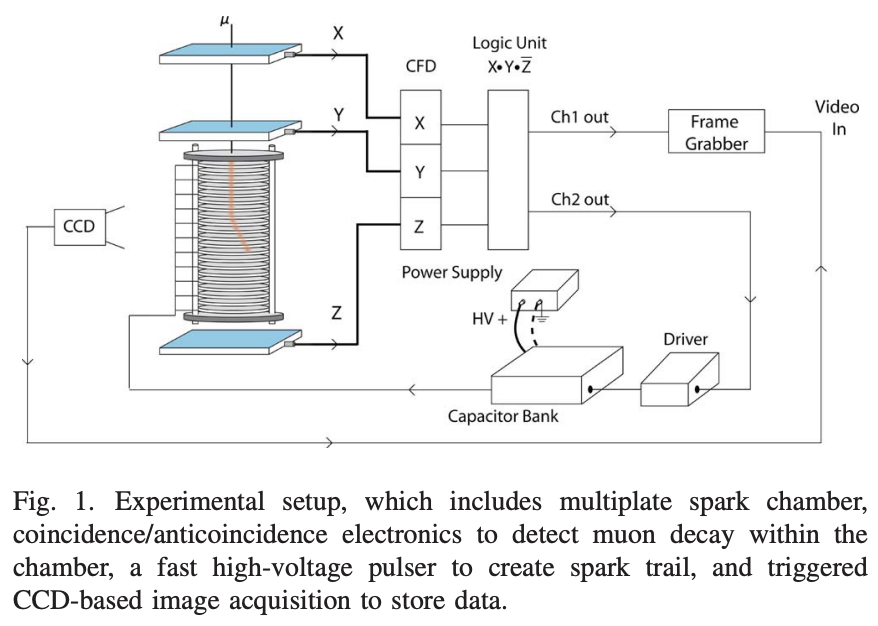
\includegraphics[width=60mm]{Fig 1.png}
    \end{figure}

    \hfil

    Figure 2: It demonstrates the spark image of a muon decay, which is observed with a direct and orthogonal view of the chamber used in the experiment. It also describes how the muon enters the chamber, together with the motion of the decay product.

    \begin{figure}[h!]
        \centering
        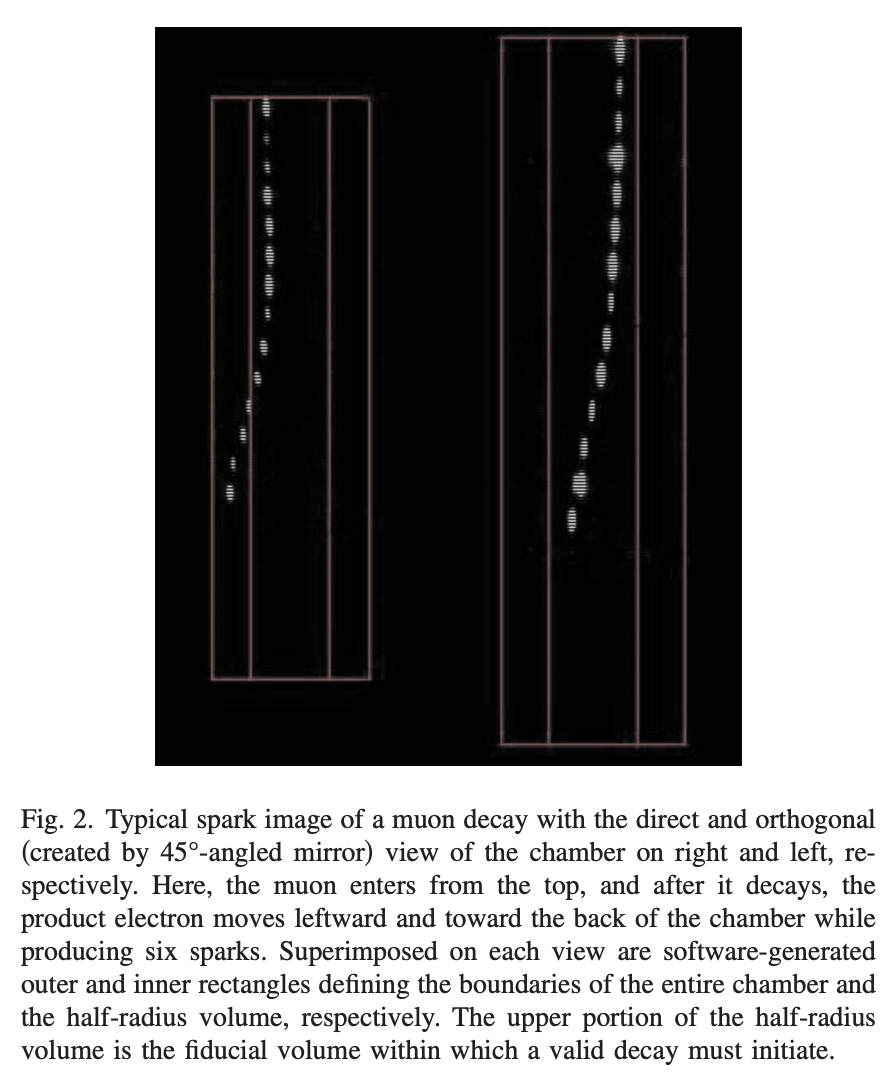
\includegraphics[width=60mm]{Fig 2.png}
    \end{figure}

    \hfil

    Figure 3: It's a histagram comparing the experimental data about the number of muon decays vs. the number of sparks observed, and the data gathered in the simulation.

    \newpage

    \begin{figure}[h!]
        \centering
        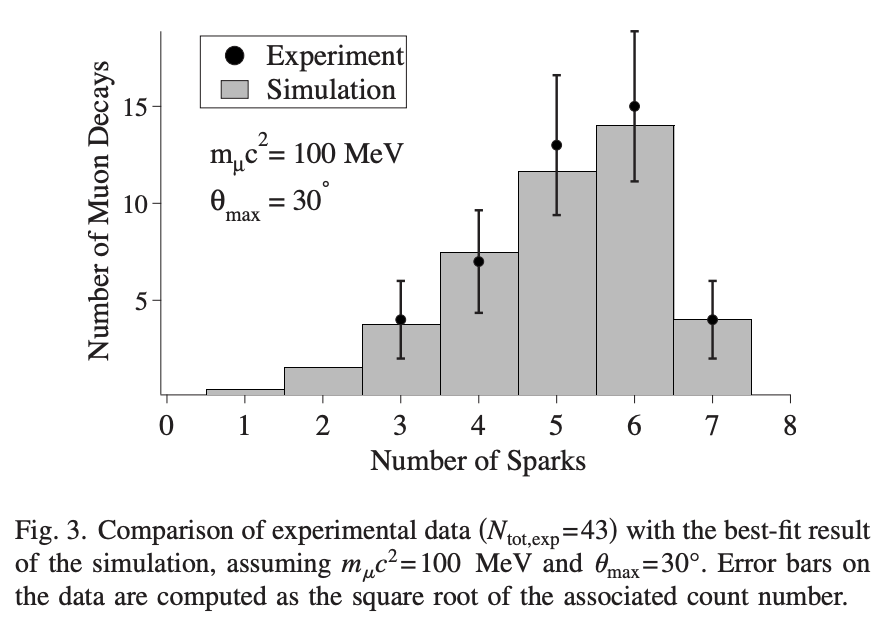
\includegraphics[width=60mm]{Fig 3.png}
    \end{figure}

    \hfil

    Figure 4: It demonstrates the geometry of the spark chamber designed in the simulation. It also shows how as the decayed electron started traveling through the chamber, how it interacts with the chamber and display the desired data.

    \begin{figure}[h!]
        \centering
        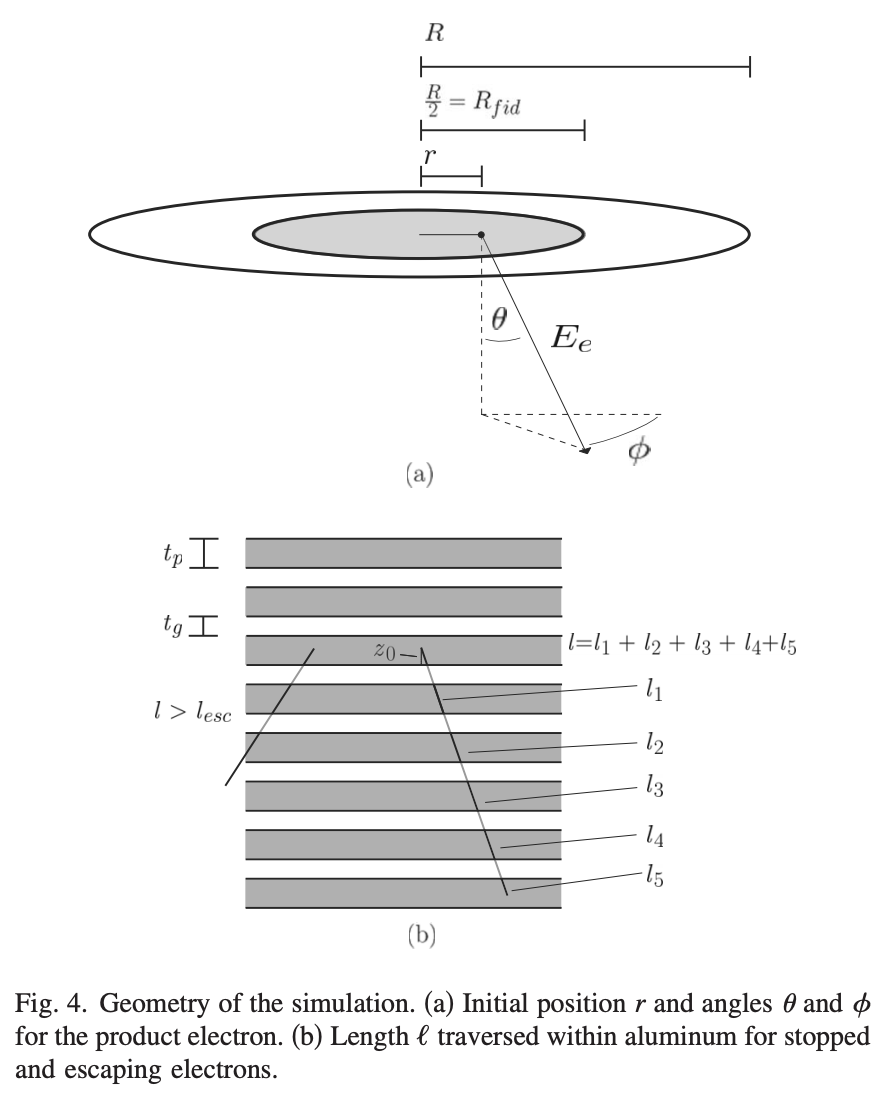
\includegraphics[width=60mm]{Fig 4.png}
    \end{figure}

    \hfil

    Figure 5: It's a graph demonstrating the relations between the rest energy of a muon, versus the sum of squared residuals (which represents the difference betwen the number of muon decays happened in the experiment vs. the simulation prediction).

    \begin{figure}[h!]
        \centering
        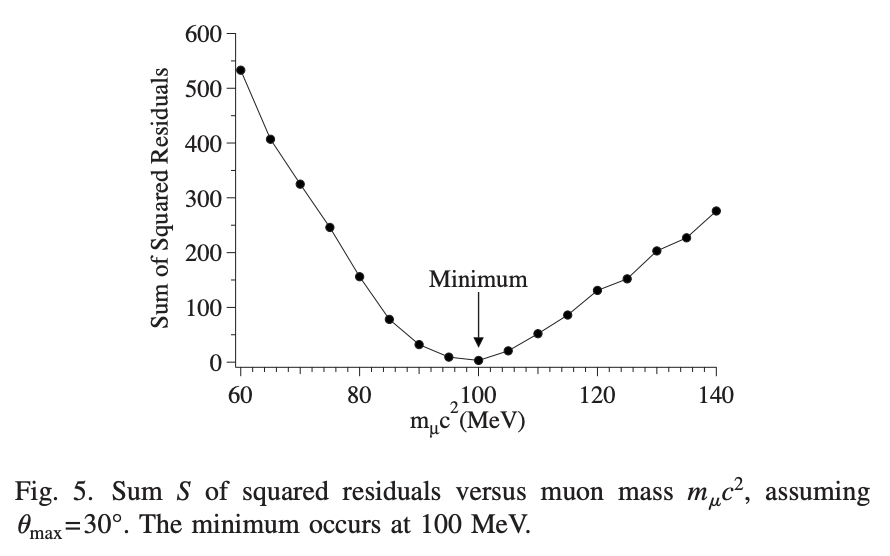
\includegraphics[width=60mm]{Fig 5.png}
    \end{figure}

    \hfil

    Figure 6: Similar to Figure 3, here it's a histgram comparing the experimental data about the number of muon days, vs. the number in simulation prediction. Except this time the rest energy of the muon is 90 MeV, instead of 100 MeV like in Figure 3.

    \begin{figure}[h!]
        \centering
        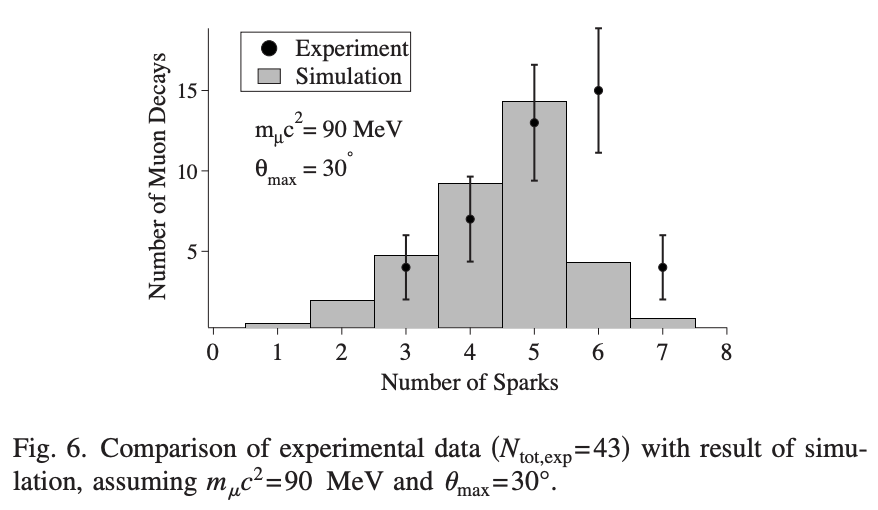
\includegraphics[width=60mm]{Fig 6.png}
    \end{figure}

    \hfil

    Figure 7: This demonstrates the design of a circuit of a capacitor bank, which is used for applying triggerable high-voltag pulses to the spark chamber.

    \begin{figure}[h!]
        \centering
        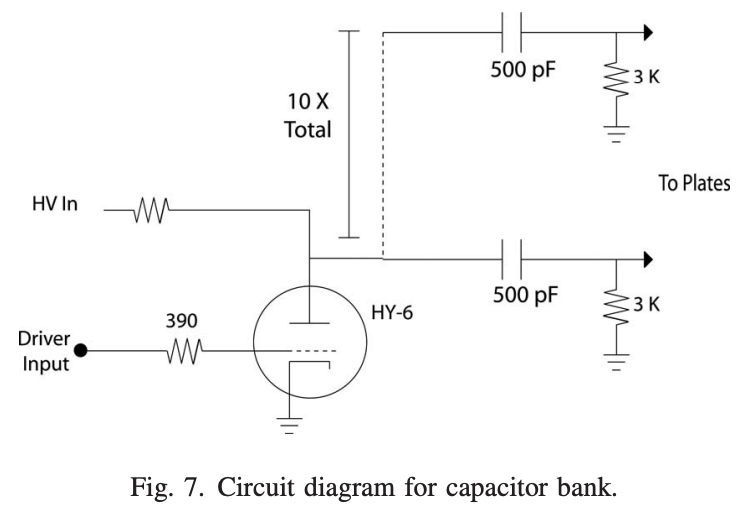
\includegraphics[width=60mm]{Fig 7.png}
    \end{figure}

    \hfil

    \item Read the paper with description of each paragraph:
    \begin{itemize}
        \item First paragraph introduces the importance of cosmic rays in particle physics studies and experiments.
        \item Second paragraph talks about high-speed muons and their presence in cosmic rays near Earth's surfaces, mentioning various effects (including time dilation) on detecting muons behavior, and also mention the history of experiments used to detect muon's masses.
        \item The third paragraph talks about the main purpose of the paper, which is a method of deriving accurate muon mass from the data collected from the mentioned experiments.
        
        \hfil

        \item The fourth paragraph talks about the details of muon as a particle, including basic properties, its potential results of its decay, while also explaining some problems faced when using the cosmic ray muons for experiments.
        \item The fifth paragraph talks about the goal of the experiment, which is stopping most of the secondary cosmic ray muons within a chamber to observe the decay of muon; it also describes the setup of the chamber used for the experiment, together with the chamber's interaction with the muons.
        \item The sixth paragraph talks about the relativistic derivation of the energy and momentum after the decay, using relativistic energy and momentum conservation.
        \item The seventh paragraph describes how together with the derived energy together with the Fermi description of muon decay, the equations could derive a bound for the mass of the muon.
        
        \hfil

        \item The eighth paragraph describes the details of the experimental system used, specifically about each components.
        \item The ninth paragraph describes a much detailed setup of the spark chamber used in the experiment, and the desired interaction happens within the chamber.
        \item The tenth paragraph describes the method of detecting the sparks happening in the chamber.
        \item The eleventh paragraph describes the method of interacting when detecting a muon passing through the chamber.
        \item The twelfth paragraph describes the method of capturing a photo and video of the spark chamber when muons are detected.
        
        \hfil

        \item The thirteenth to seventeenth paragraphs mainly described the experimental procedures, and about what data they'll record in each step.
        \item The eighteenth paragraph described some differences between the real experiment vs. their expectations.
        \item The ninteenth paragraph describes the alternative approach to data analysis due to the problems faced in the experiment.
        
        \hfil

        \item The twentieth to twenty-fourth paragraphs describes the details they used for data aalysis, and some formulas involved, and some of the resulting data value.
        
        \hfil

        \item The twenty-fifth paragraph is the conclusion, describing the experimental results and the calculation they got. 
        
        \item The twenty-sixth paragraph includes some acknowledgement about how the ideals are gotten.
        
        \hfil

        \item Finally, the twenty-seventh to thirty-second paragraphs are some details on the construction of the spark chamber.
    \end{itemize}

    Unknown words:
    \begin{itemize}
        \item Antiparticle
        \item Antineutrino
        \item antimuon
        \item Fermi description
        \item boson
    \end{itemize}

    \hfil

    \item Reflection:
    
    \begin{itemize}
        \item First, the things I learned includes some background information of muons. Also, I've learnedsome of the complications one needs to be aware of when trying to detect / do experiments about high-speed muons.
        \item Some questions I have remaining included: How are the Fermi description derived (since I don't know the results, and it provided nothing about details that I can learn). Also, I'm also curious about what causes the expectation about the observations within the spark chambers vs. what actually happened (since it wasn't fully explained). 
    \end{itemize}
\end{enumerate}

\newpage

\section*{Exercise 2}

About the paper cited in Exercise 1, here are some extra information about the citation:
\begin{enumerate}
    \item There are total of 13 papers this paper cited.
    \item A paper it cites that describes a related measurement is: "A compact apparatus for muon lifetime measurement and time dilation demonstration in the undergraduate laboratory". Unfortunately there's no references about mesauring the muon's mass, but some complications relating muon lifetime measurement (mentioned in the paper) is described here.
    \item Citation of the paper:
    
    \hfil

    Coan, Liu, Ye, "A compact apparatus for muon lifetime measurement and time dilation demonstration in the undergraduate laboratory." Am. J. Phys, 74:161-164 (2006). https://doi.org/10.1119/1.2135319 

    \hfil

    \item There are total of 4 papers that cite this paper.
    \item A paper that cites this one is: "Determining the muon mass using a scintillator-based detector." Which this also focuses on measuring muon mass.
    \item Citation of the paper:
    
    \hfil

    Woo, Essick, "Determining the muon mass using a scintillator-basd detector." Am. J. Phys. 85: 611-618 (2017). https://doi.org/10.1119/1.4984811 
\end{enumerate}

\end{document}